%%%%%%%%%%%%%%%%%%%%%% PRÉAMBULE
% !TeX program = xelatex

%%%%%%%%%%%%%% partie obligatoire du préambule
\documentclass[12pt,twoside]{book}
\usepackage{fontspec}
\usepackage{xunicode}
\usepackage{polyglossia}
\setmainlanguage{french}%indiquer la langue principale du document
%\setotherlanguage{} %indiquer les autres langues utilisée


%%%%%%%%%%%%%%%%%%%%%%%%%%%%%%%%% PACKAGES UTILISÉS
\usepackage{pdfpages}%insérer des pdf
\usepackage{csquotes} % les guillemets français
\usepackage{lettrine} %faire une lettrine (pas obligatoire)

\usepackage[style=enc,sorting=nyt,maxbibnames=10]{biblatex}%charger le style de l'EnC (téléchargeable ici https://ctan.org/pkg/biblatex-enc)
%\addbibresource{} %le fichier bibliograhique. Exemple de chemin à partir du dossier où se trouve le document maître:Exemple ./dossierA/fichier.bib
%\defbibheading{}{\subsection*{}} Si l'on veut changer le titre de la/les bibliographie(s)


%%%Faire un ou plusieurs index

%\usepackage{imakeidx} %pour faire un ou plusieurs index
%\makeindex %commande pour générer l'index


%RAJOUTEZ ICI VOS PACKAGES
\usepackage{etoolbox}\pretocmd{\part}{\setcounter{chapter}{0}}{}{}
%pour réinitialiser la numérotation des chapitres à chaque nouvelle partie. 
\usepackage{pdflscape} % Permet d'insérer des pages en orientation paysage

\usepackage{array}     % Pour \extrarowheight

%%%%%%%%%%%%%%%%%%%%%%%%%%%%%%%%% CONFIGURATION DE MISE EN PAGE

%%%%%% Les compteurs (sections, subsections, etc)


%%%%%% Les compteurs (sections, subsections, etc)
\renewcommand{\thesection}{\Roman{section}.}%On ne fait apparaître que le numéro de la section
\renewcommand{\thesubsection}{\arabic{subsection}.}%subsection en chiffres arabes
\renewcommand{\thesubsubsection}{\alph{subsubsection}.}%subsubsection en lettres minuscules
%Si l'on veut faire apparaître les subsubsection dans le table des matières (à commenter sinon)
\setcounter{tocdepth}{3}
\setcounter{secnumdepth}{3}  % La subsubsection (profondeur=3 dans la table des matières) apparait numérotée dans la TdM



%%%%%  Configurer le document selon les normes de l'école

\usepackage[margin=2.5cm]{geometry} %marges
\usepackage{setspace} % espacement qui permet ensuite de définir un interligne
\onehalfspacing % interligne de 1.5
\setlength\parindent{1cm} % indentation des paragraphes à 1 cm


%%%%% Mise en forme des headers (haut de page)

\usepackage{fancyhdr} %package utilisé pour modifier les headers
\pagestyle{fancy} %utiliser ses propres choix de mise en page et non ceux par défaut du package

\setlength\headheight{16pt}%la hauteur des headers

%%la façon dont les sections apparaissent dans les en-tête:

\renewcommand{\sectionmark}[1]{\markright{\small\textit{\thesection~\  #1}}}%Faire apparaître dans les headers les sections en  petit et en italiques
%\renewcommand{\sectionmark}[1]{}%Commenter la lign précédetne et mettre celle-ci pour ne pas avoir le titre des sections dans le header

%% réglages propres à frontmatter

\appto\frontmatter{\pagestyle{fancy}%
	\renewcommand{\chaptermark}[1]{\markboth{\small\textit{#1}}{}}% ne pas faire apparaître de <<numéro>> de chapitre dans les chapitres non numérotés (front: l'introduction, els remerciement, etc)
}

%% réglages propres à mainmatter

\appto\mainmatter{
	\renewcommand{\chaptermark}[1]{\markboth{\small\chaptername~\thechapter~--\ \textit{#1}}{}}%faire apparaître dans les headers les sections en  petit et en italiques
	%\renewcommand{\chaptermark}[1]{}%Commenter la ligne précédente et mettre celle-ci pour ne pas avoir le titre des chapitres  dans le header
}

%% réglages propres aux annexes

\appto\appendix{
	\renewcommand{\chaptermark}[1]{\markboth{\small~Annexe \thechapter~--\ \textit{#1}}{}}%faire apparaître dans les headers le nom des annexes
	%\renewcommand{\chaptermark}[1]{}%Commenter la ligne précédente et mettre celle-ci pour ne pas avoir le titre des chapitres  dans le header
}




%indiquer des règles d'hyphénation pour des mots précis si besoin
%\begin{hyphenrules}{french}
%	\hyphenation{}
%\end{hyphenrules}


%%%%%%% Package hyperref

% A mettre après les autres appels de packages car redéfinit certaines commandes).

\usepackage[colorlinks=false, breaklinks=true, pdfusetitle, pdfsubject ={Mémoire TNAH}, pdfkeywords={les mots-clés}]{hyperref} %
\usepackage[numbered]{bookmark}%va avec hyperref; marche mieux pour les signets. l'option numbered: les signets dans le pdf sont numérotés

% Compléter pdfsubjet et pdfkeywords
%Explication des options de hyperref (modifiables)
% hyperindex=false
% colorlinks=false: pour que le cadre des liens n'apparaisse pas à l'impression

% breaklinks permet d'avoir des liens allant sur pusieurs lignes
%pdfusetitle: utiliser \author et \title pour produire le nom et le titre du pdf


%avec overleaf, utiliser :
%\usepackage[xetex]{hyperref}
\hypersetup{
	pdfauthor = {Joséphine Maire},
	pdftitle = {titre},
	pdfsubject = {sujet},
	pdfkeywords = {bibliothèques} {technologies numériques appliquées à l'histoire} {école des chartes} {etc}
}










%%%%%%%%%%%%%% INFORMATIONS POUR LA PAGE DE TITRE

\author{Joséphine \textsc{Maire} - M2 TNAH}
\title{De la source musicale à la scène : structurer un projet numérique européen au service de la recherche et de l'interprétation historiquement informée. Le cas de LaDocumenta.eu .}

%%%%%%%%%%%%%%%%%%%%%% DOCUMENT
\begin{document}
	\begin{titlepage}
		\begin{center}
			
			\bigskip
			
			\begin{large}				
				ÉCOLE NATIONALE DES CHARTES\\
				UNIVERSITÉ PARIS, SCIENCES \& LETTRES
			\end{large}
			\begin{center}\rule{2cm}{0.02cm}\end{center}
			
			\bigskip
			\bigskip
			\bigskip
			\begin{Large}
				\textbf{Joséphine Maire}\\
			\end{Large}
			%selon le cas
			\begin{normalsize} \textit{licenciée ès lettres}\\
			\end{normalsize}
			
			\bigskip
			\bigskip
			\bigskip
			
			\begin{Huge}
				\textbf{De la source musicale à la scène : structurer un projet numérique européen au service de la recherche et de l'interprétation historiquement informée. Le cas de LaDocumenta.eu}\\[1.5cm]
				Volume d'annexes : livrables techniques.\par
			\end{Huge}
			
			\bigskip
			\bigskip
			\begin{LARGE}
				
			\end{LARGE}
			
			\bigskip
			\bigskip
			\bigskip
			\begin{large}
				Sous la direction de \textbf{Emmanuelle Bermès}
			\end{large}
			\vfill
			
			\begin{large}
				Mémoire 
				pour le diplôme de master \\
				\enquote{Technologies numériques appliquées à l'histoire} \\
				\bigskip
				2026
			\end{large}
			
		\end{center}
	\end{titlepage}
	
	\thispagestyle{empty}	
	\cleardoublepage
	
	\frontmatter
	
	\chapter{Résumé}
	\markboth{}
	\medskip Ce volume présente les livrables réalisés pendant un stage effectué en alternance au sein du projet LaDocumenta.eu, une bibliothèque numérique créée par un consortium d'orchestres européens de pratique historiquement informée.\\
	
	Il contient 3 livrables.\\ 
	Livrable 1 : Chartes des ressources de LaDocumenta.eu\\
	Livrable 2 : Manuel de dépôt de la plateforme LaDocumenta.eu\\
	Livrable 3 : Usages de LaDocumenta.eu et scénario d'utilisation de l'IA.\\\\
	
	\textbf{Informations bibliographiques:} Joséphine Maire, \textit{De la source musicale à la scène : structurer un projet numérique européen au service de la recherche et de l'interprétation historiquement informée. Le cas de LaDocumenta.eu. Volumes d'annexes : livrables techniques.}, mémoire de master \enquote{Technologies numériques appliquées à l'histoire}, dir. Emmanuelle Bermès, École nationale des chartes, 2026.
	
	\newpage{\pagestyle{empty}\cleardoublepage}
	

	
	

	
	%%%%%%%%%%%%%%%%%
\mainmatter


% Définition de la commande page blanche entre chaque livrable
\newcommand{\pageblanche}{%
	\clearpage
	\thispagestyle{empty}
	\mbox{}
	\clearpage
}

% 1er livrable
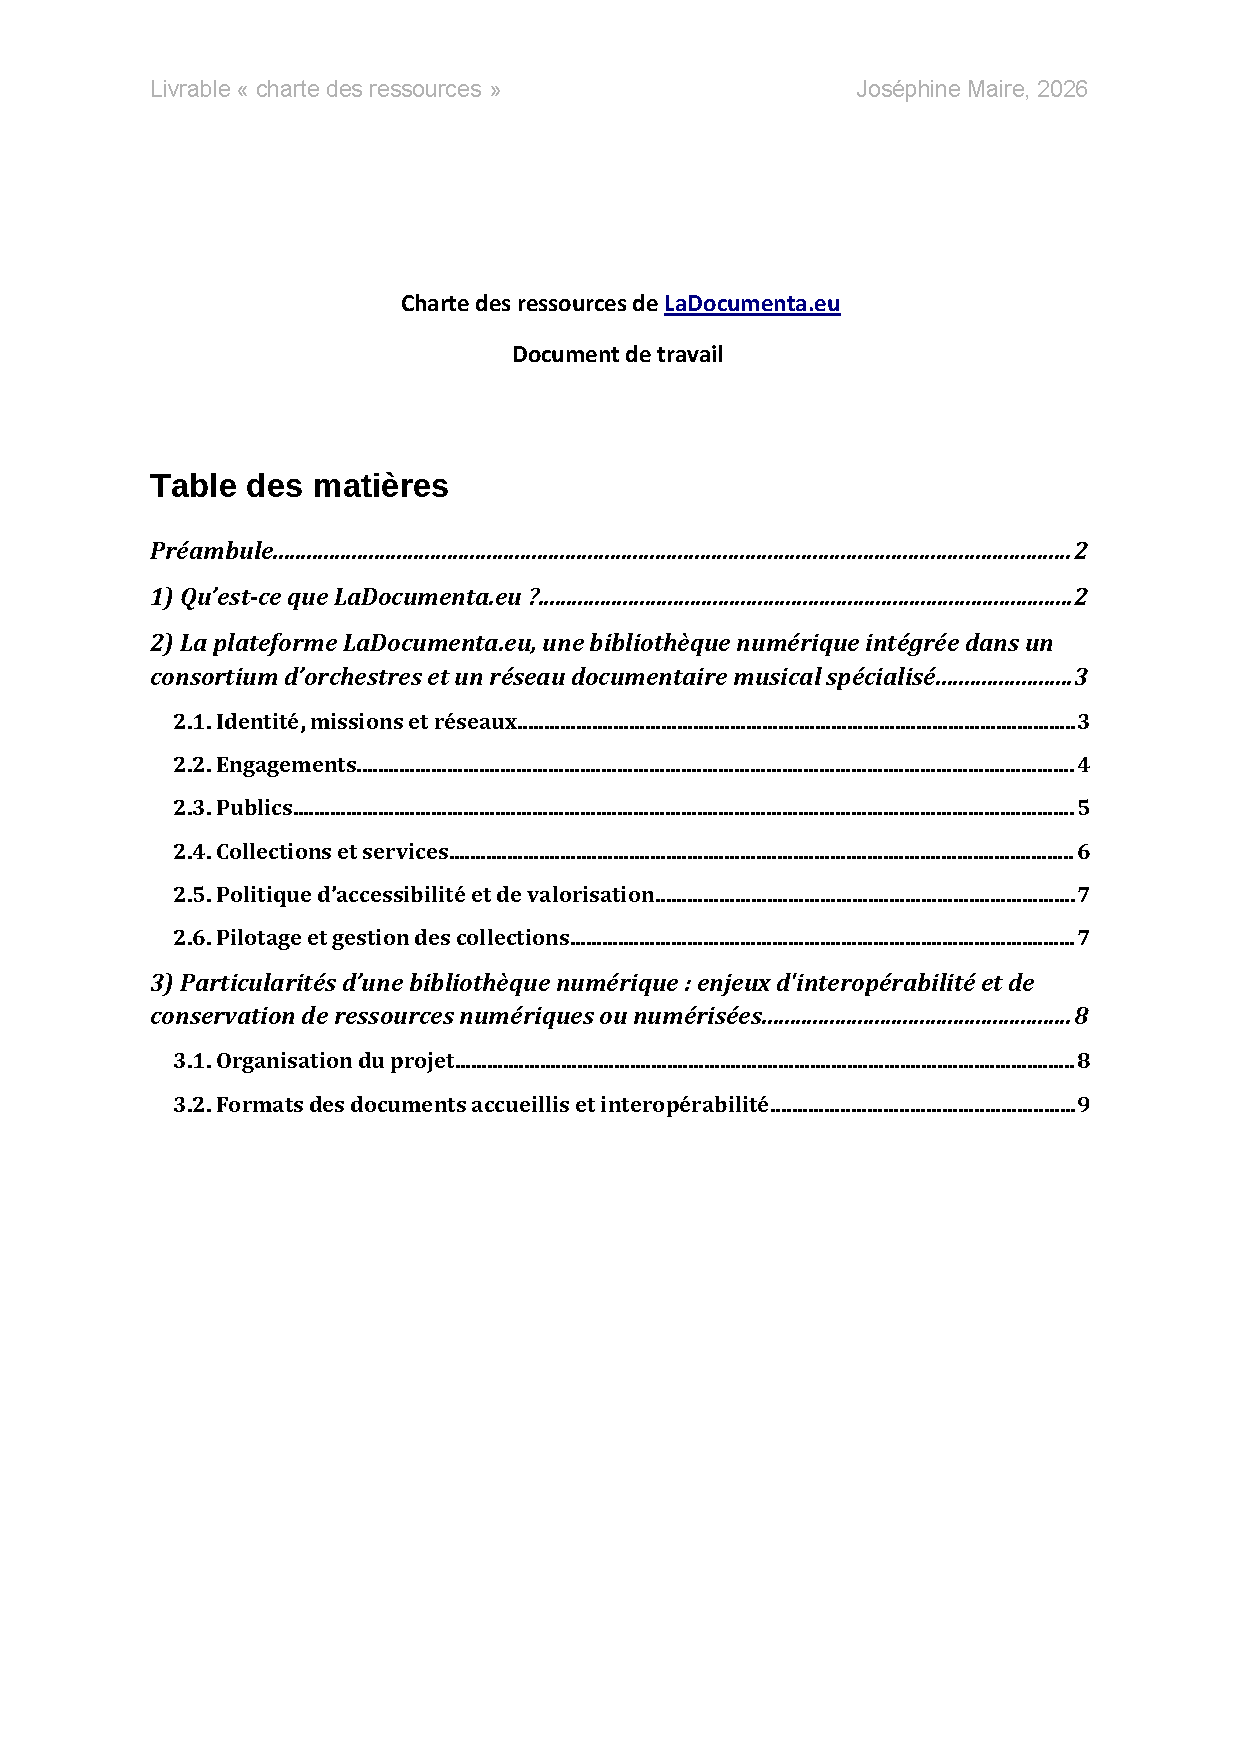
\includepdf[pages=1,
pagecommand=\subsection*{Livrable 1 : Charte des ressources de LaDocumenta.eu}]{annexe_livrable1_charte_ressources.pdf}
\includepdf[pages={2-10}]{annexe_livrable1_charte_ressources.pdf}

\pageblanche % Page blanche entre le 1er et le 2e livrable

% 2e livrable

\includepdf[pages=1, landscape=true,
pagecommand=\subsection*{Livrable 2 : Manuel de dépôt, plateforme LaDocumenta.eu}]{annexe_livrable2_manuel_depot.pdf}

\includepdf[pages={2-44}, landscape=true]{annexe_livrable2_manuel_depot.pdf}

\pageblanche % Page blanche entre le 2e et 3e livrable

% 3e livrable
% Pages 1 à 7 en portrait
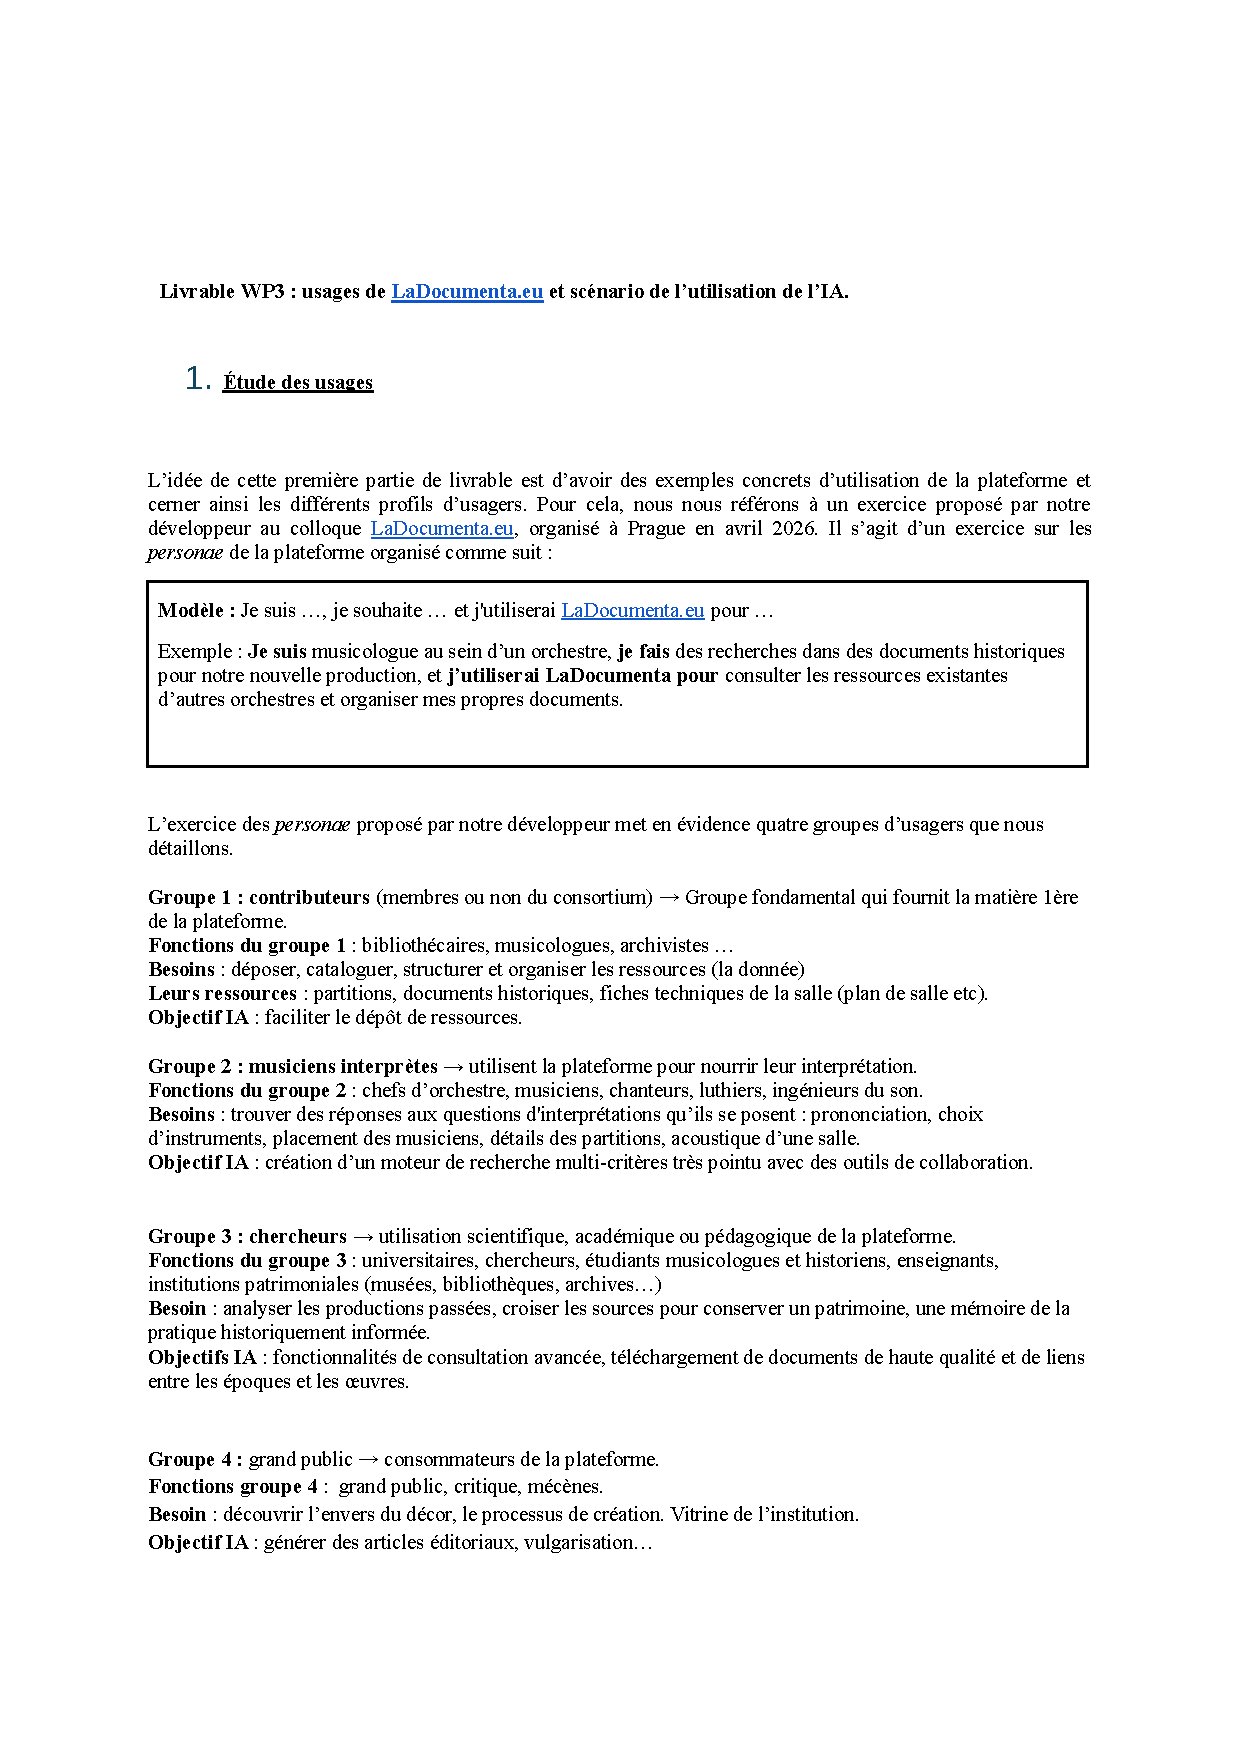
\includepdf[pages=1,
pagecommand=\subsection*{Livrable 3 : Usages de la plateforme et scénario IA.}]{annexe_livrable3_usages_ia.pdf}
\includepdf[pages={2-7}]{annexe_livrable3_usages_ia.pdf}
% Pages 8 à 12 en paysage
\includepdf[pages={8-12}, landscape=true]{annexe_livrable3_usages_ia.pdf}

\end{document}